\documentclass{article}
% --- watermark (auto-inserted) ---
\usepackage{xcolor}
\usepackage{xfp}% \fpeval; in the kernel since 2022, harmless on older LaTeX
\usepackage{draftwatermark}
\newlength{\watermarkTextWidth}
\AddToHook{begindocument/end}{%
  \SetWatermarkText{\normalfont Generated by The Agentic Scientist}%
  \SetWatermarkFontSize{10pt}%
  \SetWatermarkLightness{0.85}%
  \settowidth{\watermarkTextWidth}{\normalfont\fontsize{10pt}{12pt}\selectfont Generated by The Agentic Scientist}%
  \edef\watermarkScale{\fpeval{0.8 * sqrt(\paperwidth**2 + \paperheight**2) / \watermarkTextWidth}}%
  \edef\watermarkAngle{\fpeval{atand(\paperheight/\paperwidth)}}%
  \SetWatermarkScale{\watermarkScale}%
  \SetWatermarkAngle{\watermarkAngle}%
}
% --- end watermark ---
 % For LaTeX2e
\usepackage{paper,times}

\usepackage{hyperref}
\usepackage{url}
\usepackage{graphicx}
\usepackage{booktabs}
\usepackage{subcaption}
\usepackage{amsmath,amssymb}

\title{How Accurate Is Regression-Based Global Effect Estimation Under Network Interference? An Eight-Case Synthetic Evaluation}
\author{Anonymous authors}

\newcommand{\gate}{\mathrm{GATE}}

\begin{document}
\maketitle

\begin{abstract}
In online experiments on social networks and marketplaces, a user's outcome depends on other users' treatments, and the quantity of interest is the global average treatment effect (GATE): the mean outcome difference between treating everyone and treating no one. Regression-based estimators fit an outcome model on exposure features from one randomized experiment and difference its predictions at the all-treated and all-control corners, but how accurate they are, and what determines their error, is poorly characterized. We measure this on an eight-case synthetic grid (3000 nodes; stochastic-block, Barab\'asi--Albert and Watts--Strogatz graphs; additive, strong, saturating, degree-dependent and two-hop interference; Bernoulli and cluster assignment), scored on 24 unseen seeds. A frozen estimator that selects among 15 low-parameter exposure mappings with a BIC gate reaches a mean relative RMSE of 0.126, against 0.180 for plain linear exposure regression, 0.622 for difference-in-means, 0.994 for a neighbourhood Horvitz--Thompson estimator, and 0.045 for an oracle regression given the true mapping. Per-case error is 0.031--0.054 in the five cases whose generating form is linear in the neighbour-treated fraction, across three graph families, a threefold change in interference strength and both assignment designs, and 0.151--0.452 in the saturating, count-by-degree and two-hop cases. We hypothesize that exposure-mapping misspecification and corner extrapolation drive the larger errors, but the grid is not factorial and the estimator's per-case mapping choices were not verified, so this account is untested. Nominal 95\% intervals cover only 0.839 of the time. The evidence is limited to one graph size, case specifications shared between model selection and final scoring, and single-factor contrasts without per-case intervals.
\end{abstract}

\section{Introduction}
A/B tests on social networks and marketplaces violate the no-interference assumption: whether a user's outcome changes depends on who else is treated. The platform's decision-relevant estimand is then the \emph{global average treatment effect} (GATE), the mean over units of the difference between the outcome when all units are treated and when all are untreated. The difference-in-means (DiM) estimator, which is unbiased without interference, is systematically biased for the GATE under interference \citep{Eckles2016Design,Ugander2013GraphCluster}, and design-based alternatives such as Horvitz--Thompson (HT) estimators of neighbourhood exposure \citep{Aronow2013EstimatingAC,Ugander2013GraphCluster} avoid modelling assumptions at the price of large variance when the all-treated and all-control neighbourhood events are rare.

A model-based alternative is \emph{regression-based GATE estimation} \citep{Chin2018RegressionAF}: fit a regression of outcomes on the unit's own treatment, a summary of its neighbours' treatments (an \emph{exposure mapping}) and covariates; predict every unit's outcome under the all-treated and all-control assignments; and average the difference. This is attractive because it uses every unit rather than only those with extreme neighbourhoods. Its weakness is also visible in the construction: the two prediction points are the corners of exposure space (neighbour-treated fraction 1 and 0), which a randomized experiment with a moderate treatment probability rarely visits, so the estimate leans on the functional form of the fitted model. How accurate such estimators are in practice, which features of the mechanism, graph and design drive their error, and when they fail has not been laid out in a controlled grid.

\paragraph{Question and thesis.} We ask: in a single randomized network experiment, how accurately does a regression-based GATE estimator recover the truth, and which properties of the interference mechanism, graph and assignment design determine when it works? The measured pattern is that per-case error is low in the five cases whose generating form is linear in the neighbour-treated fraction and higher in the three cases whose form is not, with no visible degradation across graph family, interference strength (up to three times larger) or cluster-versus-Bernoulli assignment within the tested range, and that the model-based intervals undercover. A natural hypothesis, which the interference literature raises under the heading of misspecified exposure mappings and interference of unknown form \citep{Savje2023Misspecified,Savje2021Unknown}, is that accuracy depends on how well the fitted exposure mapping matches the generating mechanism. We state this as a hypothesis: the grid is not factorial, and the mapping the estimator selected in each case was not recorded in verified form.

\paragraph{What we do.} We evaluate one frozen estimator, a BIC-gated library of parametric exposure mappings with linear regression as the fallback, together with four reference estimators (difference-in-means, plain linear exposure regression, a neighbourhood HT estimator and an oracle regression using the true mapping) on a fixed eight-case grid, using 24 seeds that were not used for model selection. Figure~\ref{fig:overview} summarizes the pipeline and the grid.

\paragraph{Contributions.} (i) A transparent, scale-free protocol (relative RMSE per case, averaged over cases) with four reference estimators and three negative controls. (ii) Measured accuracy of regression-based GATE estimation across five interference forms, three graph families and two assignment designs, with single-factor case contrasts that are consistent with, but do not establish, exposure-mapping misspecification as the main error source. (iii) Negative results: nominal 95\% intervals cover 0.839 of the time, the two-hop case stays at relative RMSE 0.452 and its cause is unresolved, and two other estimator classes (a flexible ridge ensemble and a linear model with a design-weighted residual correction) scored worse than the gated library on the model-selection seeds. We make no claim of a bound, a theorem, or superiority beyond this grid; Section~\ref{sec:limits} lists what the evidence cannot support.

\begin{figure}[t]
\centering
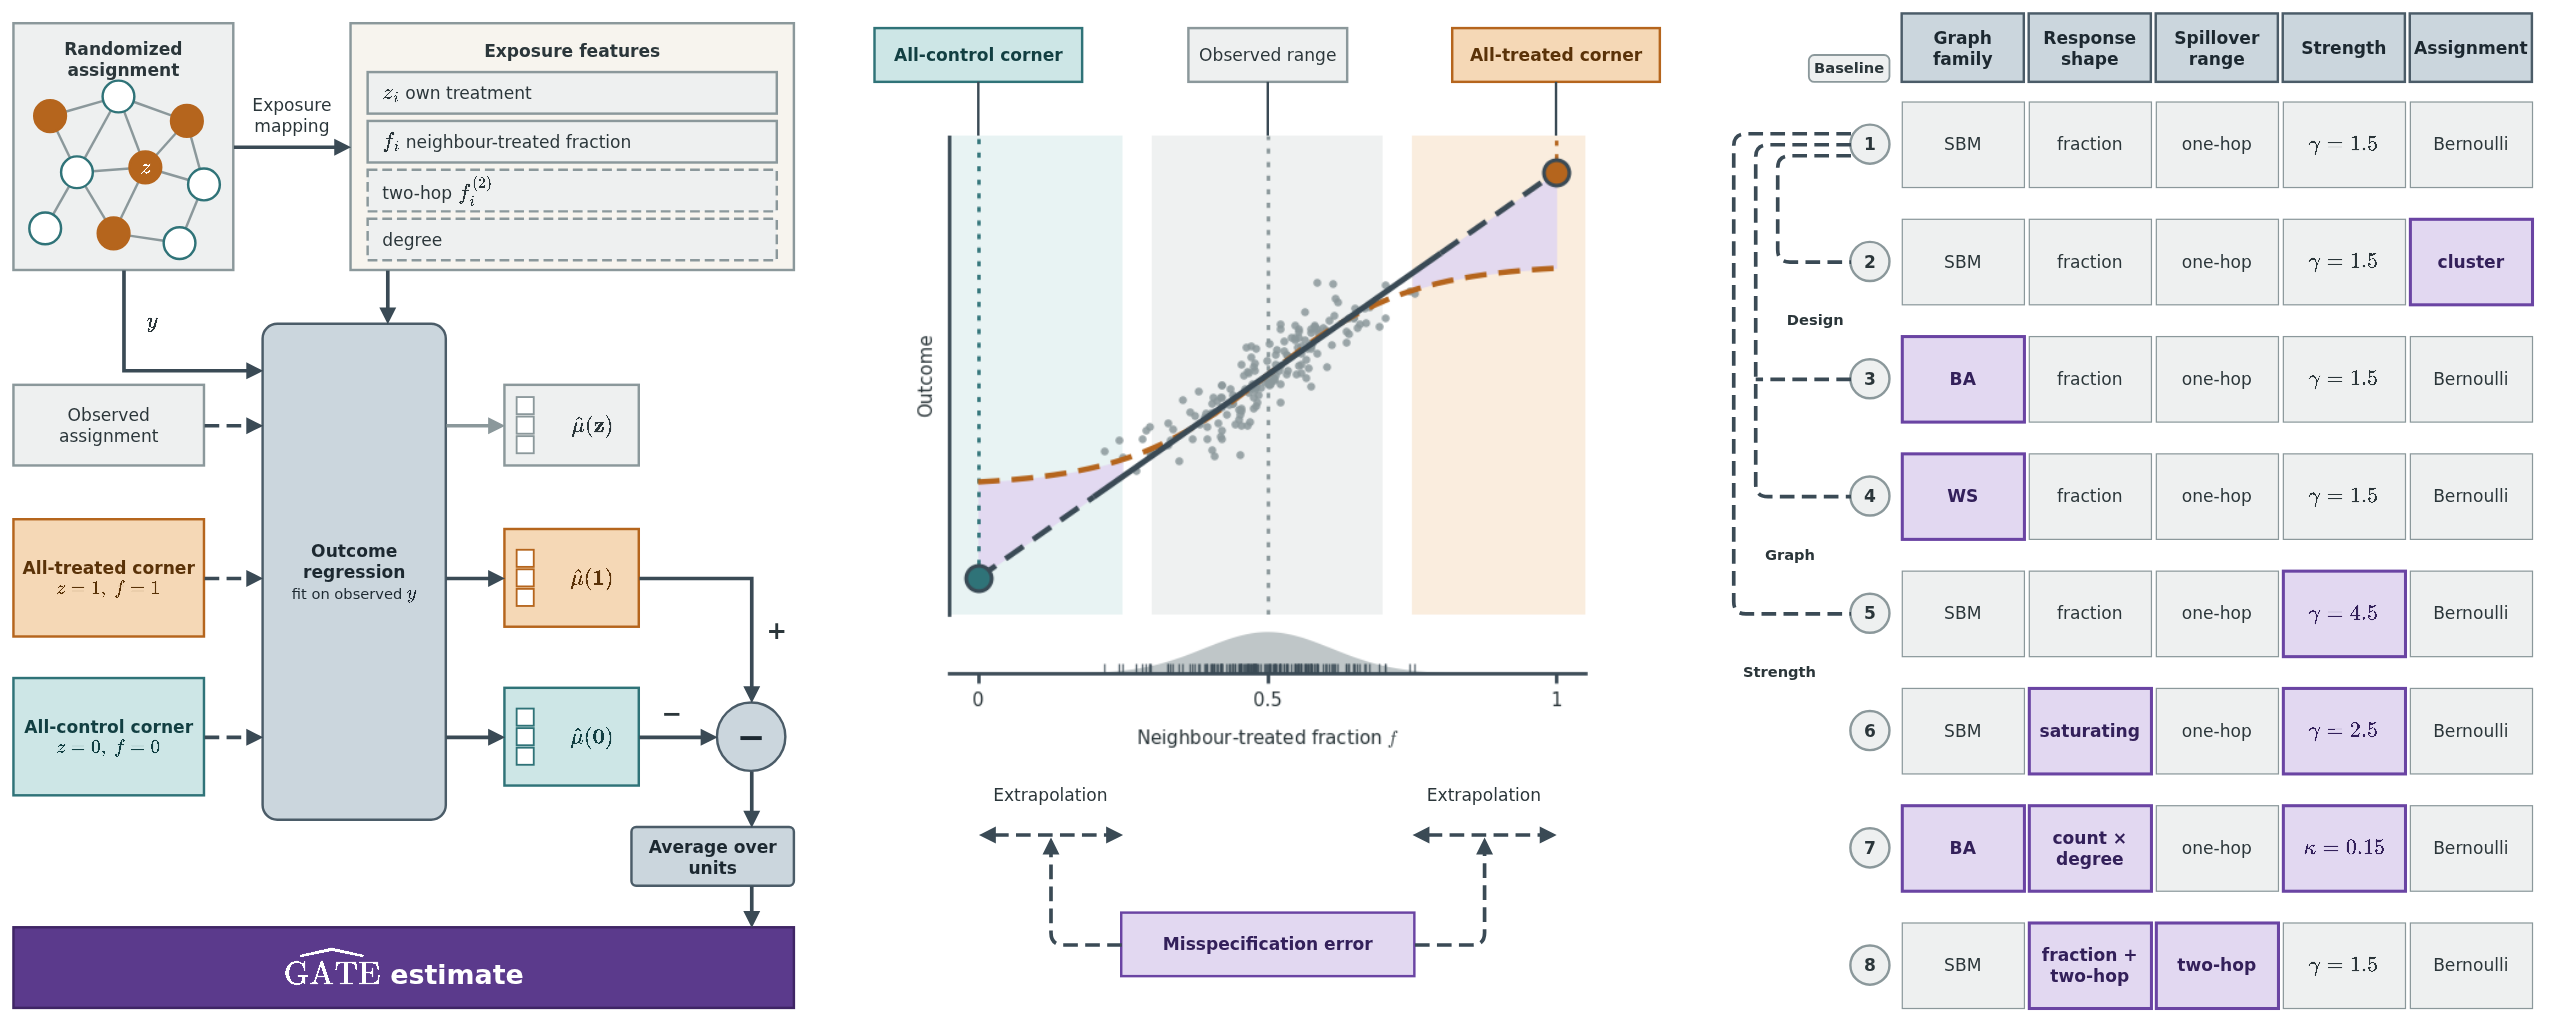
\includegraphics[width=\textwidth]{figures/overview_schematic.png}
\caption{Overview. A randomized assignment on a network yields exposure features (own treatment, neighbour-treated fraction or count, optional two-hop and degree terms); a fitted outcome regression is evaluated at the observed assignment and at the all-treated and all-control corners, and the average difference is the GATE estimate. The eight-case grid varies graph family, response shape, spillover range, strength and assignment design. Error can come from sampling noise or from misspecification of the exposure mapping, which matters most at the rarely observed corners.}
\label{fig:overview}
\end{figure}

\section{Related Work}
\paragraph{Design-based estimation under interference.} Randomization-based frameworks define exposure conditions over a network and estimate their effects with inverse-probability weighting \citep{Aronow2013EstimatingAC}; graph cluster randomization raises the probability that a unit's whole neighbourhood is treated together \citep{Ugander2013GraphCluster,Ugander2020RandomizedGC}, and it has been deployed at scale \citep{Karrer2020NetworkEA}. Subsequent work studies estimation theory under network interference \citep{Sussman2017Elements}, the admissibility of HT estimation \citep{Karwa2023Admissibility}, data-adaptive exposure thresholds for HT \citep{Thiyageswaran2024DataAdaptive}, interference with noisy or $k$-nearest-neighbour structure \citep{Li2021Noise,Alzubaidi2023KNN}, and asymptotics for effect estimation under random-graph models of the network \citep{Li2022RandomGraph}. Our HT reference is of this family; it is included as an untuned design-based reference, not as a tuned competitor.

\paragraph{Misspecified exposure mappings.} \citet{Savje2023Misspecified} treats a misspecified analyst mapping and separates the estimand's definition from the assumptions that make an estimator informative about it; \citet{Savje2021Unknown} study average-effect estimation under interference of unknown form. These works are analytical; we instead measure in a simulation grid how far a regression GATE estimator lands from the all-treated-minus-all-control contrast when the mechanism is or is not linear in the neighbour-treated fraction, and offer the corner-extrapolation account of Section~\ref{sec:corner} as a heuristic.

\paragraph{Designs for the GATE.} Several works change the assignment mechanism instead of the analysis: clustered and cluster-adaptive designs \citep{Viviano2023CausalClustering,Zhou2020ClusterAdaptive,Nandy2019Dense}, staggered or two-stage rollouts \citep{Cortez2024TwoStage}, designs matched to low-order outcome models \citep{Eichhorn2024LoworderOA}, optimized covariance of the assignment vector \citep{Chen2023OptimizedCD}, multi-arm designs under partial interference \citep{Offer-Westort2021DesigningME}, experimental design with network information \citep{Viviano2020Experimental}, and mixtures of randomized experiments \citep{Jiang2023Mixture}. We hold the two designs fixed (Bernoulli and block-cluster) and study analysis only.

\paragraph{Regression adjustment and model-based estimation.} \citet{Chin2018RegressionAF} study regression adjustments for estimating the global treatment effect under interference, by predicting outcomes in the all-treated and all-control worlds from a fitted outcome model; a related central-limit-theorem result is given by \citet{Chin2018Stein}. \citet{Han2023ModelbasedRA} propose model-based regression adjustment for network interference. Generalized propensity-score approaches model exposure probabilities \citep{Forastiere2022EstimatingCE}, and \citet{Shankar2024ABTU} and \citet{Bhattacharya2019Uncertainty} address estimation when the network is only partly known. Our contribution relative to this literature is empirical: a controlled grid that separates cases where the fitted mapping matches the mechanism from cases where it does not, with explicit reference estimators, negative controls and an interval-calibration check. We do not derive new theory.

\section{Method}
\subsection{Problem setup}
A graph $G$ on $n=3000$ nodes has adjacency $A$ and degree $d_i$. Each unit has covariates $x_i\in\mathbb{R}^2$ and a binary assignment $z_i$ drawn by the design. Outcomes follow $Y_i(\mathbf z)=\mu_i(\mathbf z)+\varepsilon_i$ with $\varepsilon_i\sim\mathcal N(0,1)$. The target is
\begin{equation}
\gate=\frac1n\sum_{i}\big[\mu_i(\mathbf 1)-\mu_i(\mathbf 0)\big].
\end{equation}
An estimator receives the graph, covariates, assignment, observed outcomes, the design description (kind, probability, cluster labels) and a nominal level of 0.95, and returns an estimate and an interval. It never sees the mechanism or the truth.

\paragraph{Metric.} The per-run error is relative, $e=\min(|\hat\tau-\gate|/|\gate|,\,2)$; instances are constructed so that $|\gate|\ge 0.5$. For each case the evaluator takes the RMSE of $e$ over seeds, and the plane score is the unweighted mean over the eight cases (``mean relative RMSE''; lower is better). We use this because GATE magnitudes differ across mechanisms and the cap of 2 keeps a high-variance estimator from dominating the average; a failed or invalid response counts as $e=2$. We also report the mean over cases of the absolute mean signed relative error (``bias''), the mean coverage of the 95\% interval, and its mean width divided by $|\gate|$ (capped at 4).

\subsection{Simulation grid}
Table~\ref{tab:cases} lists the eight cases; full parameters are in Supplementary Table~\ref{tab:spec}. The outcome mean is $\mu_i(\mathbf z)=1+x_i^\top\beta+(\tau_0+\tau_1x_{i1})z_i+h_i(\mathbf z)$ with $\beta=(0.8,-0.5)$, $\tau_0=1$, $\tau_1=0.5$ and an interference term $h_i$ built from the neighbour-treated fraction $f_i=\sum_jA_{ij}z_j/\max(d_i,1)$:
\begin{itemize}\setlength{\itemsep}{0pt}
\item \emph{fraction}: $h_i=\gamma f_i$ with $\gamma=1.5$ (cases 1--4) or $\gamma=4.5$ (case 5);
\item \emph{saturating}: $h_i=\gamma/(1+e^{-10(f_i-0.5)})$ with $\gamma=2.5$ (case 6);
\item \emph{count$\times$degree}: $h_i=0.15\,c_i\sqrt{10/\max(d_i,1)}$, $c_i=\sum_jA_{ij}z_j$ (case 7);
\item \emph{two-hop}: $h_i=1.5f_i+2.0\,f^{(2)}_i$, where $f^{(2)}_i$ is the treated fraction among nodes at distance exactly two (case 8).
\end{itemize}
Graphs are a ten-block stochastic block model (SBM; expected within-block degree 14, between-block 6), a Barab\'asi--Albert (BA) graph with $m=10$ and a Watts--Strogatz (WS) graph with $k=8$ and rewiring probability 0.1. Assignment is Bernoulli with $p=0.5$, or (case 2) five of the ten SBM blocks chosen uniformly and treated together. In SBM cases the first covariate carries a block-level shift. The graphs and truth are generated by an evaluator that is private to the estimator.

\begin{table}[t]
\centering\small
\caption{Eight-case grid and frozen-estimator error on the 24 unseen seeds (relative RMSE per case). Each factor contrast in the text is a single case pair.}
\label{tab:cases}
\begin{tabular}{clllc}
\toprule
Case & Graph & Interference form & Assignment & Rel.\ RMSE\\
\midrule
1 & SBM & fraction, $\gamma=1.5$ & Bernoulli & 0.051\\ % @evidence[[paper_data.json#final_evaluation.metrics.rmse_rel_case_1]]
2 & SBM & fraction, $\gamma=1.5$ & cluster & 0.031\\ % @evidence[[paper_data.json#final_evaluation.metrics.rmse_rel_case_2]]
3 & BA & fraction, $\gamma=1.5$ & Bernoulli & 0.054\\ % @evidence[[paper_data.json#final_evaluation.metrics.rmse_rel_case_3]]
4 & WS & fraction, $\gamma=1.5$ & Bernoulli & 0.040\\ % @evidence[[paper_data.json#final_evaluation.metrics.rmse_rel_case_4]]
5 & SBM & fraction, $\gamma=4.5$ & Bernoulli & 0.034\\ % @evidence[[paper_data.json#final_evaluation.metrics.rmse_rel_case_5]]
6 & SBM & saturating sigmoid & Bernoulli & 0.198\\ % @evidence[[paper_data.json#final_evaluation.metrics.rmse_rel_case_6]]
7 & BA & count$\times$degree & Bernoulli & 0.151\\ % @evidence[[paper_data.json#final_evaluation.metrics.rmse_rel_case_7]]
8 & SBM & fraction + two-hop & Bernoulli & 0.452\\ % @evidence[[paper_data.json#final_evaluation.metrics.rmse_rel_case_8]]
\bottomrule
\end{tabular}
\end{table}

\subsection{Compared estimators}
\paragraph{Plain linear exposure regression (baseline).} Ordinary least squares of $y$ on $[1,\,z,\,f,\,x]$, predicting at $z=\mathbf 1,\mathbf 0$ (with $f=1$ for non-isolated nodes at the all-treated corner and $f=0$ at the all-control corner). This is the canonical regression GATE estimator \citep{Chin2018RegressionAF} with a one-hop fraction mapping, as implemented by the evaluator (\texttt{source\_evidence/evaluator/evaluate.py}, \texttt{\_linear\_features} and \texttt{\_ols\_gate}). Its mapping is linear in the neighbour fraction, as is the generating term in cases 1--5; the generating own-treatment effect also includes a treatment-by-covariate interaction that this regression omits.

\paragraph{Frozen BIC-gated exposure library (studied estimator).} The studied estimator (\texttt{source\_evidence/frozen\_estimator/program.py}, functions \texttt{candidate\_designs}, \texttt{bic\_gate}, \texttt{\_estimate}) fits by least squares the linear model above plus 14 alternatives, each with few parameters: a treated-neighbour count divided by the mean degree; a two-hop walk fraction; interactions with log-degree and covariates (three variants); saturating $1-e^{-kf}$ with $k\in\{1,3,8\}$; sigmoids of $f$ centred at $\{0.25,0.5,0.75\}$ with scale 0.1; and saturating functions of the count scaled by $\{0.5,1,2\}\times$ the median degree. Exposure features are computed analytically at the observed, all-treated and all-control assignments. In the count mapping only, the all-treated feature is capped at three times the 99.5th percentile of its observed values. An alternative is kept only if its BIC is lower than the linear model's by more than 10; kept alternatives are averaged with BIC weights, and if none passes, or the average departs from the linear estimate by more than three times $\max(|\hat\tau_{\mathrm{lin}}|,\mathrm{se}_{\mathrm{lin}})$, the linear estimate is returned. The interval is $\hat\tau\pm\big(1.96\,\mathrm{se}+|\hat\tau-\hat\tau_{\mathrm{lin}}|\big)$, where $\mathrm{se}$ is the BIC-weighted mean of HC1 sandwich delta-method standard errors plus the weighted spread of the kept estimates. The estimator is deterministic, reads neither the design description nor the cluster labels, and uses no resampling. It was developed after the two earlier estimator classes had been scored on the model-selection seeds; its per-case gate decisions were not logged in verified form (the evaluation marks candidate diagnostics as unverified), so we cannot report which mapping it selected in any case. In particular, the library contains the exact sigmoid form used to generate case 6 (centre 0.5; steepness 10 corresponds to scale 0.1), so the case-6 error cannot be read as absence of the true form from the library.

\paragraph{Reference estimators (evaluator-owned).} \emph{DiM}: treated mean minus control mean. \emph{HT}: a neighbourhood-exposure Horvitz--Thompson estimator that keeps units whose closed neighbourhood is entirely treated (or entirely control) and weights by the design-implied probability of that event. \emph{Oracle}: OLS with the true exposure mapping for the case plus covariates and an own-by-covariate term; it is a reference for correct specification, not an attainable method. Definitions follow \texttt{source\_evidence/evaluator/evaluate.py} (\texttt{baseline\_dim}, \texttt{baseline\_ht}, \texttt{\_oracle\_features\_for}).

\paragraph{Negative controls.} The evaluator also sends matched requests with permuted outcomes, a node-relabelled graph and a constant outcome, and replays one episode. They are intended to probe whether the estimate reacts to scrambled graph or outcome structure and whether the estimator is deterministic.

\subsection{Protocol and scope}
Model selection used eight seeds (101--108) on the same eight case specifications; three estimator classes were each scored once there (Supplementary Table~\ref{tab:search}). One estimator was then frozen and evaluated once on 24 seeds (9001--9024) with fresh graphs and assignments, which is the evidence for all headline numbers. No invalid or failed runs occurred on the final plane. The final evaluation completed with outcome \emph{qualified}; this means the evaluator's declared requirements were met on this grid and does not by itself establish validity, generality or superiority beyond it. Because case specifications are shared between model selection and final scoring, the final gain over the linear baseline measures behaviour on new seeds of known mechanism families, not transfer to new mechanisms.

\section{Results}
\subsection{Accuracy and baselines}
\begin{figure}[t]
\centering
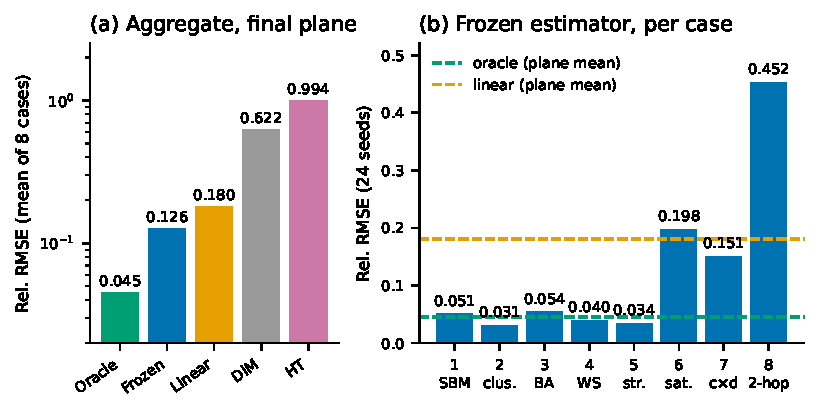
\includegraphics[width=\textwidth]{figures/main_accuracy.pdf}
\caption{Final plane, 24 unseen seeds. (a) Mean relative RMSE over the eight cases for the oracle, the frozen estimator, linear exposure regression, difference-in-means (DiM) and neighbourhood HT (log axis). (b) Frozen-estimator relative RMSE per case (SBM: Bernoulli assignment; clus.: SBM with cluster assignment; str.: strong interference; sat.: saturating; c$\times$d: count$\times$degree; 2-hop: two-hop); dashed lines are the oracle and linear plane means. Per-case values for the reference estimators are not available.}
\label{fig:main}
\end{figure}
Figure~\ref{fig:main}a gives the headline comparison. The frozen estimator attains a mean relative RMSE of 0.126 % @evidence[[paper_data.json#final_evaluation.metrics.rmse_rel]]
 versus 0.180 for plain linear exposure regression % @evidence[[paper_data.json#final_evaluation.metrics.baseline_linear_rmse_rel]]
(ratio 0.701) % @evidence[[paper_data.json#final_evaluation.metrics.ratio_to_linear_baseline]]
 and 0.622 for DiM % @evidence[[paper_data.json#final_evaluation.metrics.baseline_dim_rmse_rel]]
(ratio 0.203). % @evidence[[paper_data.json#final_evaluation.metrics.ratio_to_dim_baseline]]
 The neighbourhood HT estimator averages 0.994 % @evidence[[paper_data.json#final_evaluation.metrics.baseline_ht_rmse_rel]]
 over the capped relative-error scale, which is not usable as an estimate in this grid; we did not log the number of units with fully treated or fully control neighbourhoods, so the cause of this error (variance, sparsity of fully exposed neighbourhoods, or the cap) is not diagnosed. The oracle regression reaches 0.045, % @evidence[[paper_data.json#final_evaluation.metrics.baseline_oracle_rmse_rel]]
 so the frozen estimator remains 2.8 times above the correct-specification reference. % @evidence[[derived_stats.json#frozen_over_oracle]]
 The ordering oracle $<$ frozen $<$ linear $\ll$ DiM $<$ HT is a plane-level statement: per-case values for the baselines were not recorded, so we cannot say in which cases the linear baseline loses to the frozen estimator.

Table~\ref{tab:agg} lists the aggregate metrics.

\begin{table}[t]
\centering\small
\caption{Final-plane aggregate metrics (24 seeds $\times$ 8 cases). Bias is the mean over cases of the absolute mean signed relative error; coverage and width are for the nominal 95\% interval and are available only for the studied estimator.}
\label{tab:agg}
\begin{tabular}{lccccc}
\toprule
Estimator & Rel.\ RMSE & Ratio to linear & Bias & Coverage & Rel.\ width\\
\midrule
Oracle (true mapping) & 0.045 & 0.249 & -- & -- & --\\ % @evidence[[paper_data.json#final_evaluation.metrics.baseline_oracle_rmse_rel]]
Frozen gated library & 0.126 & 0.701 & 0.074 & 0.839 & 0.379\\ % @evidence[[paper_data.json#final_evaluation.metrics.rmse_rel]]
Linear exposure regression & 0.180 & 1 & -- & -- & --\\ % @evidence[[paper_data.json#final_evaluation.metrics.baseline_linear_rmse_rel]]
Difference-in-means & 0.622 & 3.450 & -- & -- & --\\ % @evidence[[paper_data.json#final_evaluation.metrics.baseline_dim_rmse_rel]]
Neighbourhood HT & 0.994 & 5.510 & -- & -- & --\\ % @evidence[[paper_data.json#final_evaluation.metrics.baseline_ht_rmse_rel]]
\bottomrule
\end{tabular}
\end{table}

Two aspects need qualification. First, the gap to the linear baseline is 0.054 on a plane mean, % @evidence[[derived_stats.json#frozen_vs_linear_abs_gap]]
 and the per-seed errors have a spread (Section~\ref{sec:reliability}) that is comparable to a fraction of it; we did not run a paired test. Second, all estimators run on the same 24 instances per case, so the comparison is paired by instance, but the number of seeds is modest.

\subsection{Where the error concentrates: per-case contrasts}
Figure~\ref{fig:main}b and Table~\ref{tab:cases} show that per-case error is bimodal across the eight cases. In the five cases whose generating form is a linear function of the one-hop neighbour fraction (cases 1--5), the frozen estimator's relative RMSE lies between 0.031 and 0.054. % @evidence[[derived_stats.json#cases_1_to_5_range]]
 In the three cases where the mechanism departs from that form it is 0.198 (saturating), 0.151 (count$\times$degree) and 0.452 (two-hop). We read single-factor contrasts as follows, each from one case pair, with the caveat that no per-case interval exists:
\begin{itemize}\setlength{\itemsep}{1pt}
\item \textbf{Assignment design} (case 1 vs.\ 2, same graph and mechanism): 0.051 vs.\ 0.031. Cluster assignment did not degrade accuracy; it also changes which exposure values are observed, so a difference of 0.020 should not be over-read.
\item \textbf{Graph family} (cases 1, 3, 4; same form): SBM 0.051, BA 0.054, WS 0.040. No degradation for the heavy-tailed BA graph or the near-regular WS graph.
\item \textbf{Interference strength} (case 1 vs.\ 5): tripling $\gamma$ from 1.5 to 4.5 gave 0.051 vs.\ 0.034. Relative error did not grow with strength in this range; because the error is relative to a GATE that grows with $\gamma$, a form-correct regression's relative error can shrink as the signal grows.
\item \textbf{Response shape} (case 1 vs.\ 6): the saturating mapping raises error to 0.198. The pair also differs in $\gamma$ (1.5 vs.\ 2.5), so shape is not isolated.
\item \textbf{Degree dependence} (case 3 vs.\ 7, both BA): 0.054 vs.\ 0.151, a change in mechanism form on the same graph family.
\item \textbf{Spillover range} (case 1 vs.\ 8): adding a two-hop term gives 0.452, the largest error of the grid and about 2.3 times that of the next worst case. The pair differs in total interference as well as range.
\end{itemize}
These contrasts are consistent with the hypothesis that the mismatch between the generating form and a fraction-linear mapping, rather than graph family, strength or assignment, is what moves the error, and they do not support a simple story in which heavier-tailed degree distributions or stronger spillovers alone degrade regression GATE estimation in this range. They do not establish it: the grid is not factorial, the three cases with higher error are also the three that depart from the linear fraction form, each pair changes more than one property at a time in at least two instances, and we did not record which mapping the estimator selected, so a mapping mismatch is not shown for any case. Case 6 is a caution: the library contains its exact generating sigmoid, yet the error is 0.198, so a missing mapping alone cannot explain it; failure of the gate to select that mapping, averaging over several mappings, or finite-sample variance at the corners are all possible and untested. The oracle's plane mean of 0.045 is similar to the per-case errors in cases 1--5, suggesting residual sampling noise at $n=3000$, though this compares a plane mean with per-case values.

\subsection{A heuristic account of the corner extrapolation}\label{sec:corner}
The pattern in Table~\ref{tab:cases} can be read through a simple account that we offer as interpretation, not as a tested mechanism. Least squares fits the outcome surface where the data are: with Bernoulli assignment at $p=0.5$, a node of degree $d$ has neighbour fraction $f_i$ concentrated near 0.5 with spread of order $\sqrt{0.25/d}$, so observed exposures cover the middle of $[0,1]$ much more densely than the corners $f=0$ and $f=1$ at which the GATE is evaluated. If $h$ is linear in $f$, the fitted slope is the same everywhere and the corner prediction is correct up to sampling error. If $h$ is nonlinear, the fitted slope is a local average of $h'$ over the observed range and the corner contrast $h(1)-h(0)$ is replaced by that slope times the corner distance, which is wrong by an amount that depends on how $h'$ differs between the middle and the ends of the range. For the sigmoid in case 6 (centre 0.5, steepness 10) the slope is largest at the middle, exactly where the data lie, so a linear fit would extrapolate a steep local slope to the corners; whether the gated estimator used a sigmoid or fell back to linear in this case is not known. For the two-hop case, an exposure mapping that omits the second-hop term loses a component of the effect that is entirely absent from $f$, while for count$\times$degree interference the bias depends on how the count scales with degree across nodes. Under this account, graph family and assignment design matter only through how well the observed exposure distribution covers the corners and through noise; cluster assignment widens that coverage, a possible reason for the lower error in case 2. We did not measure corner coverage, so these statements remain hypotheses.

\subsection{Bias, variance and the model-selection comparison}
The mean absolute relative bias on the final plane is 0.074, % @evidence[[paper_data.json#final_evaluation.metrics.bias_rel_abs_mean]]
 which is 0.588 of the mean relative RMSE. % @evidence[[derived_stats.json#bias_over_rmse]]
 Per-case bias is not recorded, so a substantial systematic component exists on average but is not shown to be concentrated in the cases with higher error.

\begin{table}[t]
\centering\small
\caption{Model-selection plane (8 seeds 101--108, same eight case specifications, different seeds): plane-mean relative RMSE for the three estimator classes, each scored once. These are selection-set numbers, not final evidence; per-case values, baselines, bias and coverage for this plane are not used here.}
\label{tab:search}
\begin{tabular}{lc}
\toprule
Estimator class & Plane-mean rel.\ RMSE\\
\midrule
Flexible ridge ensemble & 0.232\\ % @evidence[[paper_data.json#grounding_sources.result.improvement_001]]
Linear + design-weighted residual correction & 0.185\\ % @evidence[[paper_data.json#grounding_sources.result.improvement_002]]
BIC-gated exposure library (selected) & 0.140\\ % @evidence[[paper_data.json#grounding_sources.result.improvement_003]]
\bottomrule
\end{tabular}
\end{table}

Table~\ref{tab:search} compares the three estimator classes on the eight model-selection seeds. The gated library has the lowest plane-mean error (0.140), against 0.185 for the linear model with a design-weighted, shrunk corner-residual correction and 0.232 for a flexible ridge ensemble with extrapolation-aware averaging. Because the evaluator's per-case and baseline values for this plane are not part of the verified evidence we use, we draw no per-case or baseline-relative conclusion from it, and in particular we do not say here whether the two alternatives beat plain linear regression. The three classes differ in several respects at once (model family, selection rule, interval construction), so this comparison supports a ranking of the three configurations on these seeds and no attribution to any single component. The library did contain a two-hop walk-fraction mapping, and the final-plane error in the two-hop case remains 0.452; why it did not resolve case 8 is \emph{unknown}. The two-hop feature in the source counts length-two walks, including walks that return to the node, and so differs from the generating distance-exactly-two fraction; whether this matters, whether the gate ever selected it, and whether the all-treated corner is poorly constrained were not tested. No ablation of the gate margin or library components was run.

\subsection{Reliability: seed variability and interval coverage}
\label{sec:reliability}
\begin{figure}[t]
\centering
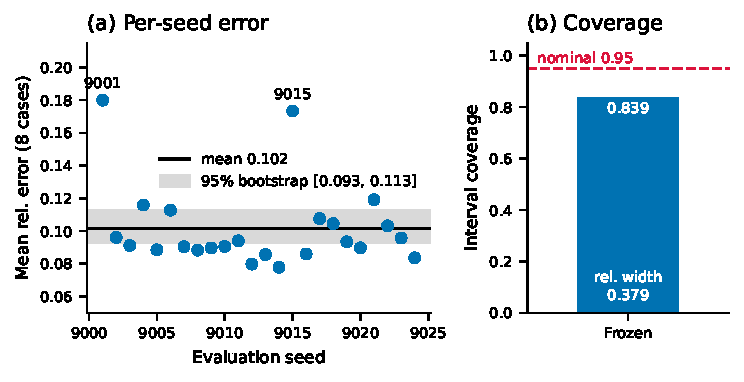
\includegraphics[width=0.72\textwidth]{figures/reliability.pdf}
\caption{(a) Per-seed mean relative error over the eight cases for the 24 final seeds, with the mean and a 95\% percentile-bootstrap interval for the mean (10{,}000 resamples over seeds). (b) Mean 95\%-interval coverage over cases against the nominal level, with mean relative interval width.}
\label{fig:rel}
\end{figure}
Per-seed errors (Figure~\ref{fig:rel}a) have a mean of 0.102 with bootstrap interval [0.093, 0.113]; % @evidence[[derived_stats.json#seed_mean]]
 this is the mean absolute relative error over cases and is lower than the RMSE aggregate of 0.126; we did not decompose the gap by case. Two seeds stand out (9001 and 9015, with per-seed errors 0.180 and 0.173), while every other seed lies between 0.078 and 0.119; % @evidence[[derived_stats.json#outlier_seeds]]
 excluding them the mean is 0.095. % @evidence[[derived_stats.json#mean_excluding_outliers]]
 Per-case decomposition for those seeds is not available, so we do not know which case drove them.

The nominal 95\% intervals covered the truth at a rate of 0.839 averaged over cases, % @evidence[[paper_data.json#final_evaluation.metrics.ci_coverage]]
 with mean relative width 0.379 % @evidence[[paper_data.json#final_evaluation.metrics.ci_width_rel]]
 (Figure~\ref{fig:rel}b). This is undercoverage by 0.111 % @evidence[[derived_stats.json#coverage_shortfall]]
 on the plane mean. The interval is built from HC1 sandwich errors for a fixed library, widened by the departure from the linear estimate; it does not model selection uncertainty beyond that spread, treats units as independent in the sandwich estimate even under the cluster design, and uses no resampling (\texttt{source\_evidence/frozen\_estimator/program.py}, \texttt{sandwich\_se}, \texttt{\_estimate}). Variance and interval estimation under network dependence is treated in the design-based literature \citep{Aronow2013EstimatingAC}, in work on regression adjustment \citep{Han2023ModelbasedRA} and in random-graph asymptotics \citep{Li2022RandomGraph}; the interval here does not follow those approaches, and we did not run any of them on this grid, so we cannot say whether they would restore nominal coverage. We report the undercoverage as an observed outcome; per-case coverage is not recorded, and we do not attribute the shortfall to a specific cause.

\subsection{Validity checks}
The constant-outcome control returned estimates with maximum absolute value $9.0\times10^{-15}$, % @evidence[[paper_data.json#final_evaluation.metrics.control_constant_max_abs_est]]
 so the estimator returned an essentially zero estimate when the outcome carried no signal. With permuted outcomes the mean absolute estimate was 0.059 of the true GATE, % @evidence[[paper_data.json#final_evaluation.metrics.control_permuted_outcome_mean_abs_rel_est]]
 and with a node-relabelled graph the relative RMSE was 0.627, % @evidence[[paper_data.json#final_evaluation.metrics.control_permuted_graph_rmse_rel]]
 which is similar to the difference-in-means value of 0.622 and much larger than the 0.126 headline. % @evidence[[paper_data.json#final_evaluation.metrics.baseline_dim_rmse_rel]]
 We do not interpret the similarity mechanistically. No control was vacuous, the replayed episode agreed exactly, and no episode failed. % @evidence[[paper_data.json#final_evaluation.metrics.replay_abs_diff]]

\section{Discussion and Limitations}
\label{sec:limits}
\paragraph{What the evidence supports.} On this grid, the frozen regression GATE estimator is accurate (relative RMSE 0.031--0.054 per case at $n=3000$) in the five cases whose generating form is linear in the neighbour fraction, across the three graph families, a threefold change in interference strength and both assignment designs. In the saturating, count$\times$degree and two-hop cases the per-case error is 0.198, 0.151 and 0.452. Whether this reflects exposure-mapping misspecification, as the literature on misspecified mappings would suggest, is a hypothesis: we did not verify which mapping was selected in any case, and case 6 shows that the library's containing the true form does not guarantee a low error. We do not extrapolate beyond the tested regime.

\paragraph{Relation to design-based estimation.} The HT reference is design-based, whereas the regression estimators accept model risk in exchange for using every unit. In this grid at $n=3000$ the HT reference scored a mean relative RMSE of 0.994 (Table~\ref{tab:agg}); we did not diagnose the cause (variance, sparsity of fully exposed neighbourhoods, or the error cap), and regression errors were larger in cases 6--8 without our having verified the cause. This does not imply that regression dominates design-based approaches: we compared analyses under two fixed designs, did not tune HT (for instance with exposure thresholds as in \citealp{Thiyageswaran2024DataAdaptive}), and did not vary graph density or size. % @evidence[[paper_data.json#final_evaluation.metrics.baseline_ht_rmse_rel]]

\paragraph{Threats to validity.} The library includes the exact case-6 sigmoid and saturating and count-based shapes close to the grid's other forms, so the gain over linear regression may partly reflect the library containing shapes close to the grid's mechanisms; this was not tested, and no ablation or per-case gate logging exists. A practitioner whose true mechanism lies outside the library would not be protected by the gate; the fallback is then plain linear regression. Relative error divides by $|\gate|\ge0.5$ and is capped at 2.

\paragraph{Limitations.} (1) Case specifications are shared between model selection and final scoring, and the library was developed after the two earlier estimator classes had been scored on the model-selection seeds; the final result is out-of-sample over seeds but not over mechanisms. (2) There is a single graph size ($n=3000$) and a single assignment probability (0.5). (3) Contrasts are single case pairs, not a factorial design; they are not accompanied by per-case intervals, and several pairs vary more than one property. (4) Per-case values for the baselines, the bias, and the coverage are unavailable, so we make no per-case baseline comparison. (5) The cause of the larger errors in cases 6--8 (including the two-hop failure) and of the undercoverage is not established, and the mapping selected per case was not verified, so the mapping-mismatch account is a hypothesis. (6) There was no ablation of the gate margin or library components, so we cannot attribute the gain over linear regression to any particular mapping or to the gate itself; only three estimator classes were scored once on the model-selection seeds, and their per-case results are not used. (7) All mechanisms are synthetic; we ran no experiment on public graphs (e.g., Facebook100), real outcomes, learned graph representations, or other designs. (8) Qualification of the final evaluation is a statement about the measured result on this grid.

\section{Conclusion}
We measured how well a regression-based GATE estimator recovers the truth under network interference on an eight-case synthetic grid. Relative RMSE was 0.031--0.054 per case in the five cases whose generating form is linear in the neighbour-treated fraction, regardless of graph family, a threefold increase in interference strength, or cluster versus Bernoulli assignment, and 0.198, 0.151 and 0.452 in the saturating, count-by-degree and two-hop cases. A BIC-gated library of parametric mappings lowered mean relative RMSE to 0.126 from 0.180 for plain linear regression, but remained 2.8 times above an oracle given the true mapping, did not fix the two-hop case, and produced intervals that cover only 0.839 of the time. We hypothesize that exposure-mapping mismatch and extrapolation to the all-treated and all-control corners drive the larger errors; this account is consistent with the single-factor contrasts but untested, because the grid is not factorial and the selected mappings were not verified. These findings are limited to one graph size, one treatment probability, and case specifications shared with model selection. Next steps are a factorial extension with per-case intervals, a gate and library ablation with logged mapping choices, and calibrated intervals.

% IMPORTANT: \clearpage flushes all pending floats before references so that
% body-page counting excludes reference-only pages.  Do NOT remove.
\clearpage
\bibliography{references}
\bibliographystyle{paper}

\clearpage
\appendix
\section{Supplementary Information}

\subsection{Simulation Design and Case Specifications}
Table~\ref{tab:spec} gives the parameters read from the case-specification file used on the final plane; model-selection seeds used the same eight specifications. Instances are generated from seeded random streams keyed by seed, graph family and node count. The evaluator requires $|\gate|\ge0.5$ and a 95\% nominal interval level. Covariates are standard normal; in SBM cases the first covariate gets an additional block-level shift of scale 0.5.
\begin{table}[h]
\centering\small
\setlength{\tabcolsep}{4pt}\footnotesize
\caption{Case specifications (all cases: $n=3000$, $\sigma=1$, intercept 1, $\beta=(0.8,-0.5)$, $\tau_0=1$, $\tau_1=0.5$).}
\label{tab:spec}
\begin{tabular}{clll}
\toprule
Case & Graph parameters & Interference parameters & Design\\
\midrule
1 & SBM, 10 blocks, deg$_{in}$ 14, deg$_{out}$ 6 & fraction, $\gamma=1.5$ & Bernoulli, $p=0.5$\\
2 & same as 1 & fraction, $\gamma=1.5$ & cluster, $p=0.5$\\
3 & BA, $m=10$ & fraction, $\gamma=1.5$ & Bernoulli, $p=0.5$\\
4 & WS, $k=8$, rewire 0.1 & fraction, $\gamma=1.5$ & Bernoulli, $p=0.5$\\
5 & same as 1 & fraction, $\gamma=4.5$ & Bernoulli, $p=0.5$\\
6 & same as 1 & sigmoid, $\gamma=2.5$, steepness 10, centre 0.5 & Bernoulli, $p=0.5$\\
7 & BA, $m=10$ & count$\times$degree, $\kappa=0.15$, $m_{ref}=10$ & Bernoulli, $p=0.5$\\
8 & same as 1 & fraction + two-hop, $\gamma=1.5$, $\gamma_2=2.0$ & Bernoulli, $p=0.5$\\
\bottomrule
\end{tabular}
\end{table}

\subsection{Estimator and Baseline Definitions}
\paragraph{Feature maps of the library.} With $f$ the one-hop treated fraction, $s$ the treated-neighbour count, $f^{(2)}$ the two-hop walk fraction (length-two walks from the node that end at a treated node, divided by all length-two walks from the node, so walks returning to the node are included), $\ell=\log(1+d)$ centred, and $\bar x$ centred covariates, the 15 mappings are: linear $[1,z,f,x]$; count $[1,z,s/\bar d,x]$; two-hop $[1,z,f,f^{(2)},x]$; interactions $[1,z,f,x,\ell,z\ell,z\bar x,f\ell]$, $[1,z,f,x,\ell,z\ell,f\ell]$ and $[1,z,f,x,f\bar x]$; saturating $[1,z,1-e^{-kf},x]$; sigmoid $[1,z,(1+e^{-(f-t)/0.1})^{-1},x]$; and saturating-count $[1,z,1-e^{-s/(k\,\mathrm{med}_d)},x]$, where $\mathrm{med}_d$ is the median degree over non-isolated nodes; the count mapping uses $s/\bar d$ with $\bar d$ the mean degree. Source: \texttt{source\_evidence/frozen\_estimator/program.py} (\texttt{\_exposure\_states}, \texttt{candidate\_designs}, \texttt{\_fit\_candidate}, \texttt{bic\_gate}, \texttt{\_estimate}). All-treated values are the analytic corner values (for example $f=\mathbf 1[d>0]$, $s=d$, $f^{(2)}=\mathbf 1[\text{walks}>0]$). The BIC is $n\log(\mathrm{RSS}/n)+p\log n$ with $p$ the rank of the design. The sigmoid with $t=0.5$ and scale 0.1 equals the case-6 generating sigmoid up to the coefficient $\gamma$, which the regression absorbs.

\paragraph{Fallbacks.} If the linear fit fails or any step raises, the estimator returns linear OLS with an HC1 interval; when the outcome variance is exactly zero the estimate is 0 with a degenerate interval.

\paragraph{Reference estimators.} DiM, linear and oracle regressions follow Section~3 (\texttt{source\_evidence/evaluator/evaluate.py}); HT uses inclusion probabilities $p^{|N_i|}$ and $(1-p)^{|N_i|}$ for Bernoulli designs, with $|N_i|=d_i+1$, and a hypergeometric probability over blocks touched by the closed neighbourhood for the cluster design. The oracle features are $[1,z,x_1,x_2,zx_1]$ (covariates $x_1,x_2$) plus the true mapping ($f$; $f$ and $f^{(2)}$; the sigmoid with true centre and steepness; or $c\sqrt{m_{ref}/d}$).

\subsection{Per-Seed Final Results}
Table~\ref{tab:seeds} lists the 24 final seeds. The per-seed value is the mean relative error over the eight cases; runtime per seed (four estimate calls per case) ranged from 9.1 to 10.9 seconds, with median 10.4. % @evidence[[derived_stats.json#median_duration_seconds]]
\begin{table}[h]
\centering\small
\caption{Final per-seed mean relative error over the eight cases (seeds 9001--9024).}
\label{tab:seeds}
\begin{tabular}{cccccccccccc}
\toprule
9001&9002&9003&9004&9005&9006&9007&9008&9009&9010&9011&9012\\
0.180&0.096&0.091&0.116&0.089&0.113&0.090&0.088&0.090&0.091&0.094&0.080\\ % @evidence[[paper_data.json#final_evaluation.evaluation_evidence.episodes]]
\midrule
9013&9014&9015&9016&9017&9018&9019&9020&9021&9022&9023&9024\\
0.086&0.078&0.173&0.086&0.108&0.105&0.093&0.090&0.119&0.103&0.096&0.084\\ % @evidence[[paper_data.json#final_evaluation.evaluation_evidence.episodes]]
\bottomrule
\end{tabular}
\end{table}
The mean is 0.102, the standard deviation 0.026 and the median 0.092. % @evidence[[derived_stats.json#seed_std]]

\subsection{Negative Controls and Determinism Checks}
\begin{table}[h]
\centering\small
\caption{Final-plane validity checks for the frozen estimator.}
\label{tab:controls}
\begin{tabular}{lr}
\toprule
Check & Value\\
\midrule
Constant outcome, max $|$estimate$|$ & $9.0\times10^{-15}$\\ % @evidence[[paper_data.json#final_evaluation.metrics.control_constant_max_abs_est]]
Permuted outcomes, mean $|$estimate$|/|\gate|$ & 0.059\\ % @evidence[[paper_data.json#final_evaluation.metrics.control_permuted_outcome_mean_abs_rel_est]]
Node-relabelled graph, relative RMSE & 0.627\\ % @evidence[[paper_data.json#final_evaluation.metrics.control_permuted_graph_rmse_rel]]
Vacuous controls & 0\\ % @evidence[[paper_data.json#final_evaluation.metrics.control_vacuity_violations]]
Replay absolute difference & 0\\ % @evidence[[paper_data.json#final_evaluation.metrics.replay_abs_diff]]
Missing or failed episodes & 0\\ % @evidence[[paper_data.json#final_evaluation.metrics.missing_or_failed_episodes]]
\bottomrule
\end{tabular}
\end{table}
The constant-outcome control returns an estimate of magnitude about $9\times10^{-15}$ (numerically zero), the permuted-outcome control gives a mean absolute estimate of 0.059 times the true GATE, and the relabelled-graph error (0.627) is far above the headline error of 0.126 and similar to the difference-in-means value. We make no mechanistic claim from these values. None of these supports accuracy on its own.

\subsection{Model-Selection Comparison of Estimator Classes}
Main-text Table~\ref{tab:search} reports the eight model-selection seeds (101--108) on the same eight case specifications. The three estimator classes were each scored once; the final estimator was frozen from this comparison, so these numbers are a selection set, not final evidence. Only the plane-mean scores are used in this paper; per-case, bias, coverage and baseline values for this plane are not reported. The two alternatives, as implemented in \texttt{source\_evidence/estimator\_01/program.py} and \texttt{source\_evidence/estimator\_02/program.py}, are: (i) a flexible ensemble that fits ridge regressions on exposure features, compares candidates by cross-validation and a held-out extrapolation split, averages those within one standard error, and builds an interval from a design-resampling wild block bootstrap; and (ii) a linear-regression estimate plus a shrunk, degree-stratified HT-type residual correction with a design-based variance term. We did not inspect their per-case behaviour, so we offer no explanation for their scores.

\subsection{Reproducibility Notes}
The directory \texttt{source\_evidence/} holds the three estimator source files (\texttt{frozen\_estimator}, \texttt{estimator\_01}, \texttt{estimator\_02}), the evaluator scripts for the two planes, both case-specification files and the evaluator's requirements file (numpy 2.2.6, scipy 1.15.3, scikit-learn 1.6.1, networkx 3.4.2). \texttt{build\_figures.py} reads the evidence registry and regenerates Figures~\ref{fig:main} and~\ref{fig:rel} and the derived statistics (bootstrap with fixed seed 0). Table~\ref{tab:cases} and Table~\ref{tab:spec} come from the final case-specification file and the evaluator's per-case metrics; Table~\ref{tab:seeds} comes from the per-seed evidence file; Table~\ref{tab:search} uses the plane scores of the three model-selection runs. Each final seed took about ten seconds on CPU. The final evaluation used seeds 9001--9024; model selection used 101--108. The overview figure in the main text is a schematic and contains no measured values.

\subsection{LLM Usage}
Large language models were used throughout this study. They proposed the three estimator classes compared on the model-selection seeds, wrote the estimator source code for them, produced the figures and analysis scripts, retrieved and screened the cited literature, and drafted this manuscript. All reported numbers come from a fixed evaluator code base run on the estimator source files, and from analysis scripts that read those outputs; no number was produced by a language model without a corresponding file. The estimator's per-case behaviour and mapping choices were not inspected beyond the recorded metrics, as noted in the limitations.

\end{document}
